\documentclass[a4paper,12pt]{article}
\usepackage[dutch]{babel}
\usepackage[utf8x]{inputenc}
\usepackage{amsmath, epic, eepic, float, subfig, amsfonts, color, amsthm, textcomp, microtype, fullpage}
\usepackage[parfill]{parskip}
\usepackage[pdftex]{graphicx}
\usepackage{color}
\usepackage[linkcolor=black,urlcolor=blue,citecolor=black]{hyperref}
\hypersetup{colorlinks=true}
\newcommand{\HRule}{\rule{\linewidth}{0.5mm}}

\begin{document}
\begin{titlepage}
\begin{center}

\includegraphics[width=0.5\textwidth]{./logo.pdf}~\\[1cm]


\textsc{\Large User Experience Design}\\[0.5cm]

\HRule \\[0.4cm]
{ \LARGE \bfseries Drop je spruit}\\[0.4cm]
{\large \emph{een alternatieve manier voor babysitting}}\\[0.2cm]

\HRule \\[1.5cm]

\begin{minipage}{0.4\textwidth}
\begin{flushleft} \large
\emph{door:}\\
Haroen \textsc{Viaene}\\

\end{flushleft}
\end{minipage}
\begin{minipage}{0.4\textwidth}
\begin{flushright} \large
\large{2$^{\text{de}}$ fase bachelor Elektronica-ICT}\\
\end{flushright}
\end{minipage}

\vfill

{\large 2015-2016}

\end{center}
\end{titlepage}

\newpage

\tableofcontents

\newpage
\begin{abstract}
We willen een toepassing ontwerpen waarmee gebruikers elkaar kunnen vinden om hun kind(eren) bij elkaar voor een korte of langere periode achter te kunnen laten. Het is bedoeld als alternatief voor babysits: in plaats van een babysit in huis te halen, worden de kinderen dus elders gebracht en weer afgehaald door de ouders. Dit kan voor een paar uur (b.v. om rustig boodschappen te kunnen doen), voor een nacht of voor meerdere dagen. Er mag door het ontvangend gezin geen vergoeding gevraagd worden.

Bedenk ook een business model: hoe kunnen wij als webbeheerders hier geld aan verdienen?
\end{abstract}

\section{Storyboard}

\begin{figure}[H]
  \centering
  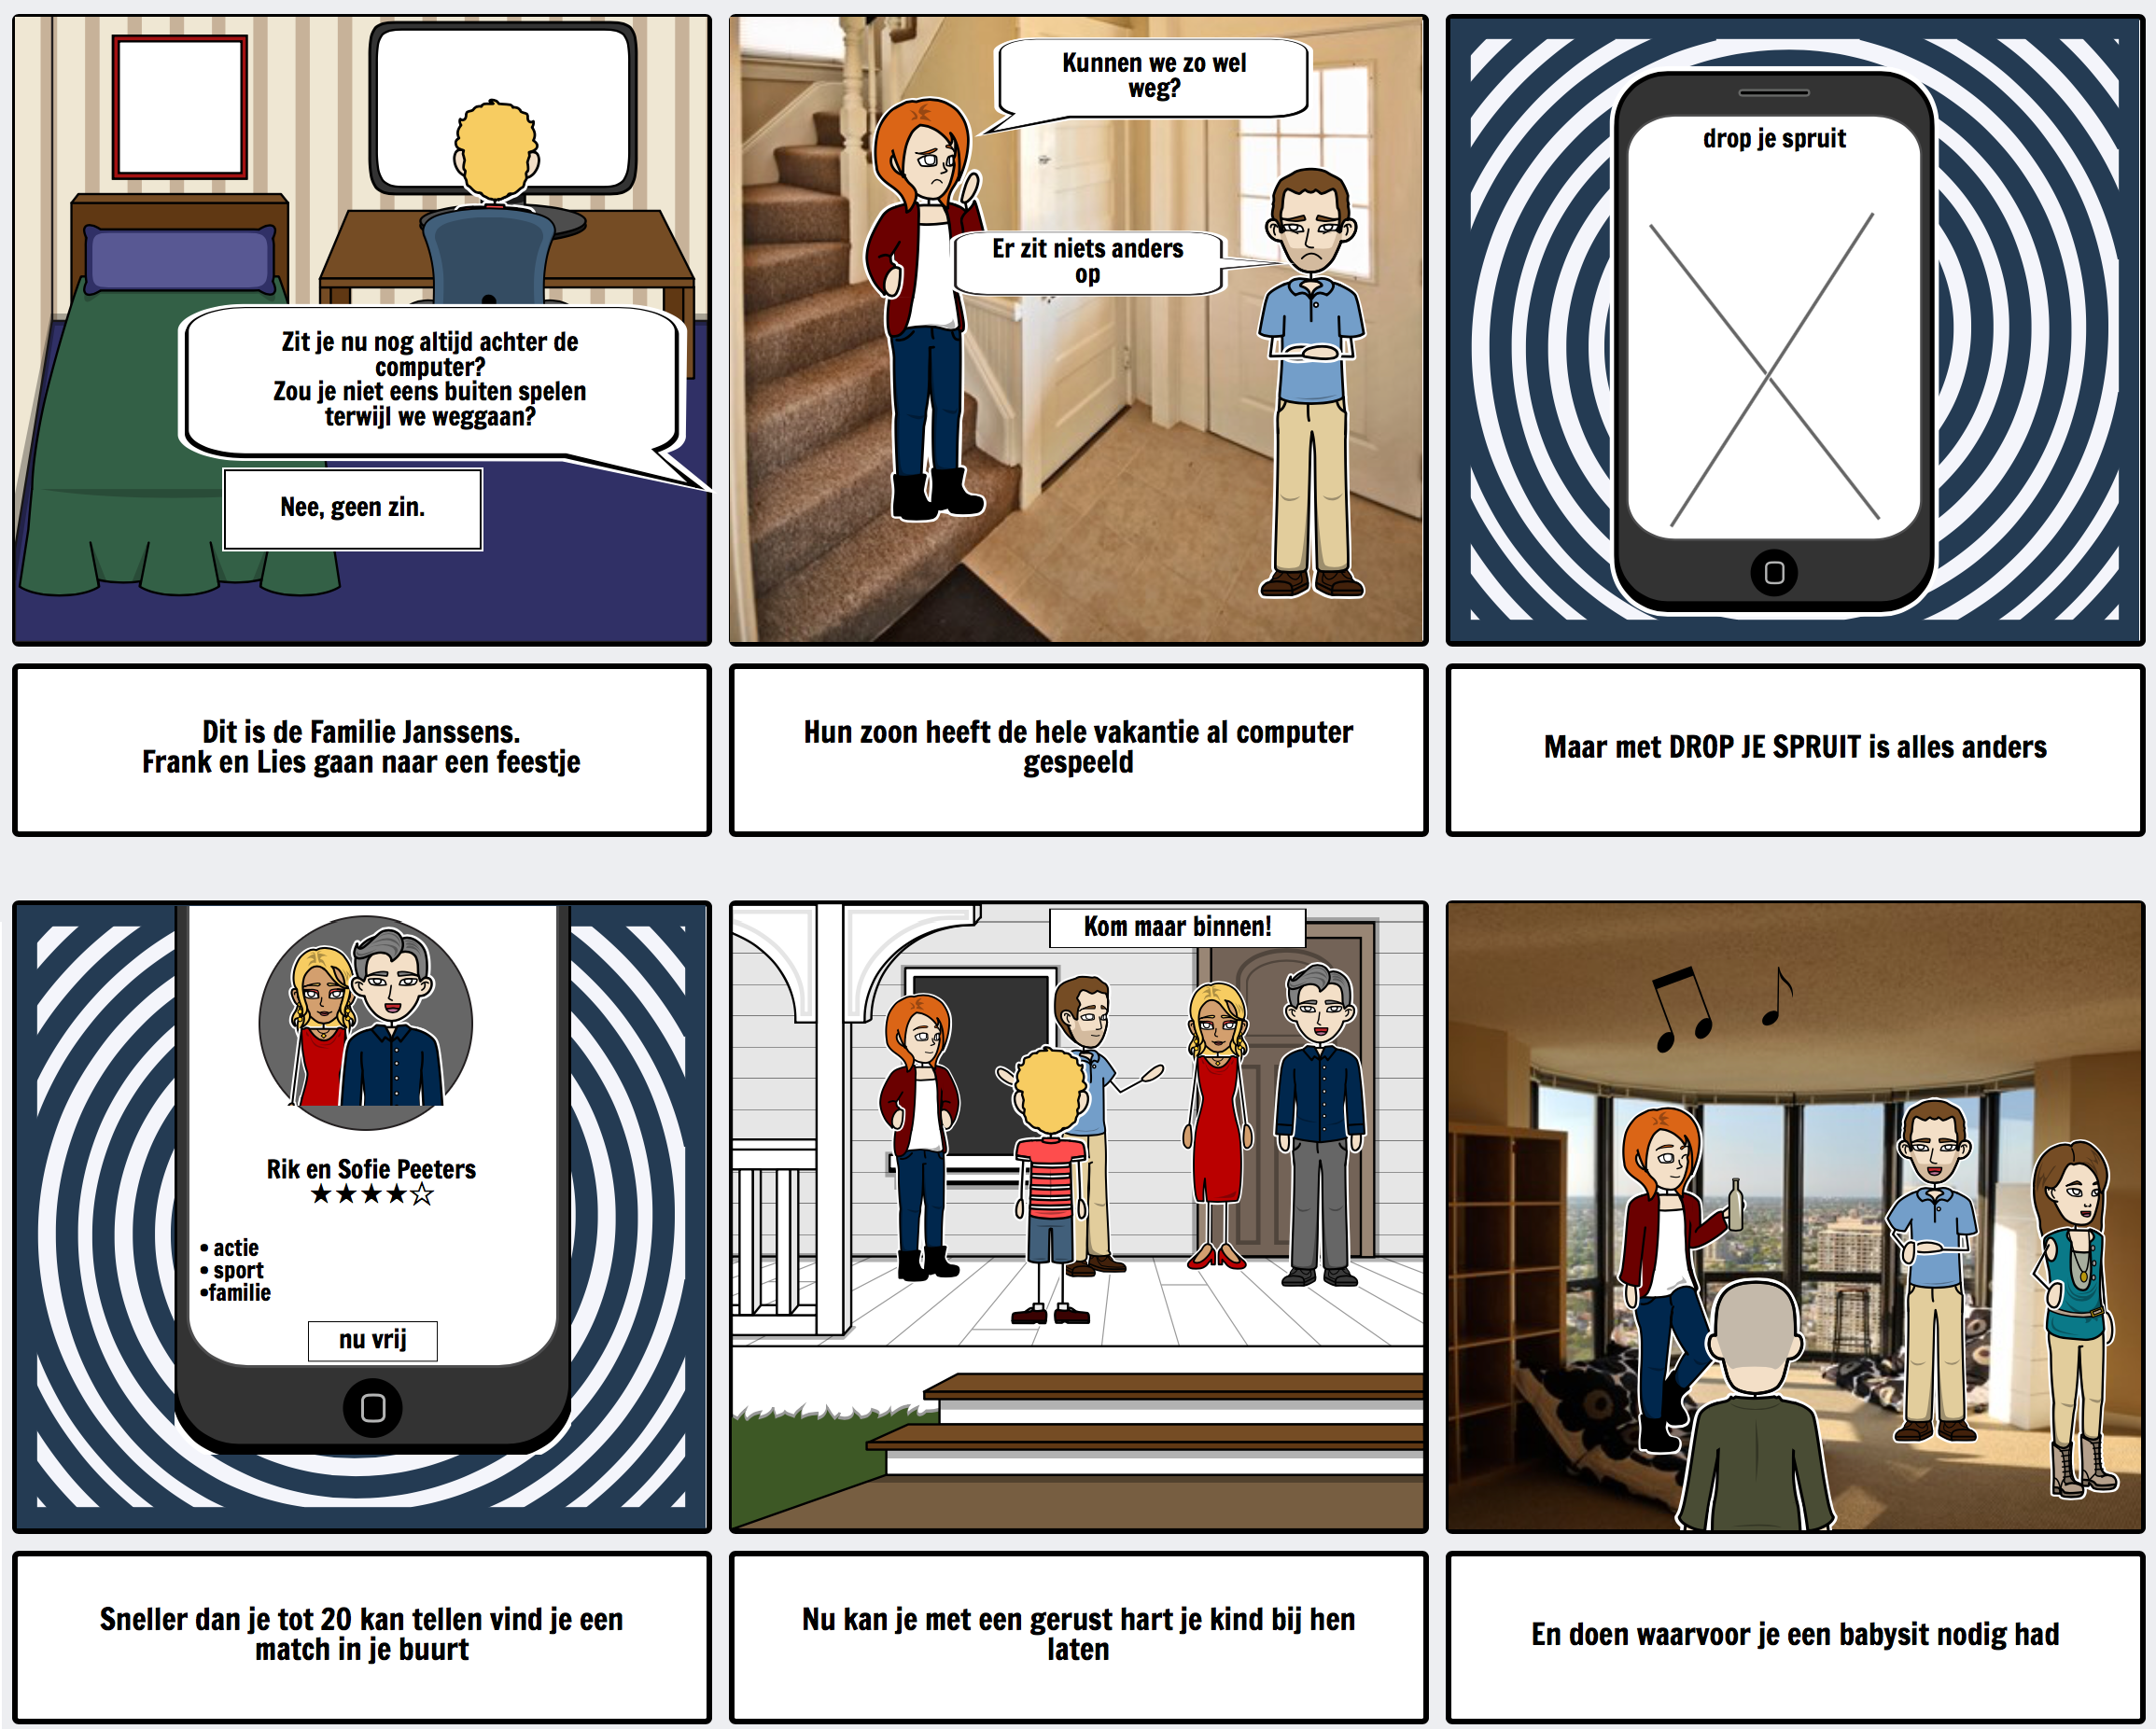
\includegraphics[width=\textwidth,keepaspectratio]{./storyboard.png}
\end{figure}

\section{Veldonderzoek}

\subsection{Vragen}
\begin{enumerate}
  \item Wie paste er laatst op je kinderen?
  \item Heb je ooit op iemand anders' kinderen gepast?
  \item Om welke redenen zijn je kinderen niet bij altijd bij je?
  \item
  \item
  \item
  \item
  \item
  \item
  \item
\end{enumerate}

\subsection{Antwoorden}

\section{Personas}

\section{Brainstorm}

\section{Scenario}

\section{Website table}

\section{Page tables}

\section{Schetsen}

\section{Prototype}

\end{document}